% !Mode:: "TeX:UTF-8" 

\BiSection{3.29}{Figures}

\fancyhead[R]{本题3.29由QC.Z完成}

解:

$M_1,M_2$是NMOS,$M_3,M_4$是PMOS

考虑电路中偏置电压和阈值电压的关系

		\begin{figure}[H] %H为当前位置,!htb为忽略美学标准,htbp为浮动图形
	\begin{minipage}{\linewidth}
		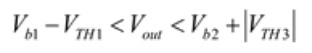
\includegraphics{3.29-1}
	\end{minipage}
\end{figure}

		\begin{figure}[H] %H为当前位置,!htb为忽略美学标准,htbp为浮动图形
	\begin{minipage}{\linewidth}
		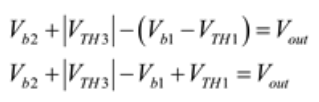
\includegraphics{3.29-2}
	\end{minipage}
\end{figure}

		\begin{figure}[H] %H为当前位置,!htb为忽略美学标准,htbp为浮动图形
	\begin{minipage}{\linewidth}
		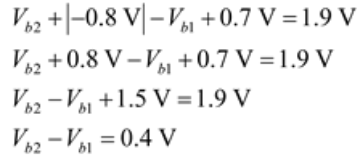
\includegraphics{3.29-3}
	\end{minipage}
\end{figure}

		\begin{figure}[H] %H为当前位置,!htb为忽略美学标准,htbp为浮动图形
	\begin{minipage}{\linewidth}
		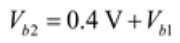
\includegraphics{3.29-4}
	\end{minipage}
\end{figure}





四个器件宽长比相同

		\begin{figure}[H] %H为当前位置,!htb为忽略美学标准,htbp为浮动图形
	\begin{minipage}{\linewidth}
		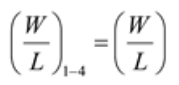
\includegraphics{3.29-5}
	\end{minipage}
\end{figure}




由$M_1$

		\begin{figure}[H] %H为当前位置,!htb为忽略美学标准,htbp为浮动图形
	\begin{minipage}{\linewidth}
		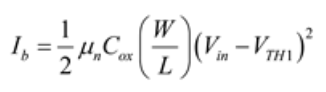
\includegraphics{3.29-6}
	\end{minipage}
\end{figure}

		\begin{figure}[H] %H为当前位置,!htb为忽略美学标准,htbp为浮动图形
	\begin{minipage}{\linewidth}
		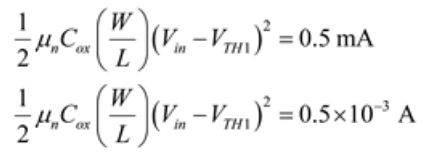
\includegraphics{3.29-7}
	\end{minipage}
\end{figure}

		\begin{figure}[H] %H为当前位置,!htb为忽略美学标准,htbp为浮动图形
	\begin{minipage}{\linewidth}
		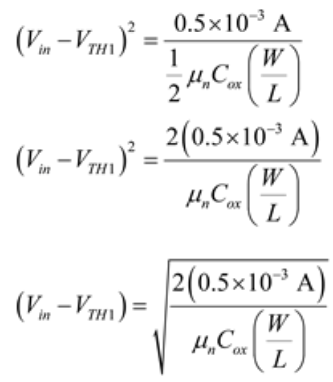
\includegraphics{3.29-8}
	\end{minipage}
\end{figure}

设$M_1,M_2$之间为X点,由$M_2$

		\begin{figure}[H] %H为当前位置,!htb为忽略美学标准,htbp为浮动图形
	\begin{minipage}{\linewidth}
		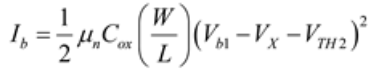
\includegraphics{3.29-9}
	\end{minipage}
\end{figure}

		\begin{figure}[H] %H为当前位置,!htb为忽略美学标准,htbp为浮动图形
	\begin{minipage}{\linewidth}
		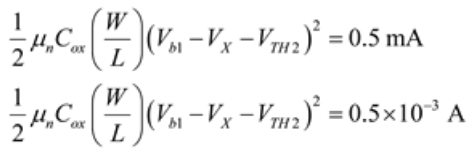
\includegraphics{3.29-10}
	\end{minipage}
\end{figure}

		\begin{figure}[H] %H为当前位置,!htb为忽略美学标准,htbp为浮动图形
	\begin{minipage}{\linewidth}
		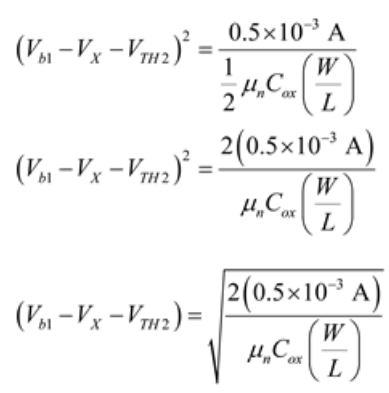
\includegraphics{3.29-11}
	\end{minipage}
\end{figure}

设$M_3,M_4$之间为Y点,由$M_3$

		\begin{figure}[H] %H为当前位置,!htb为忽略美学标准,htbp为浮动图形
	\begin{minipage}{\linewidth}
		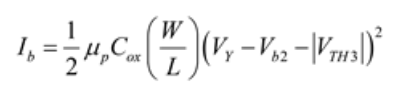
\includegraphics{3.29-12}
	\end{minipage}
\end{figure}


		\begin{figure}[H] %H为当前位置,!htb为忽略美学标准,htbp为浮动图形
	\begin{minipage}{\linewidth}
		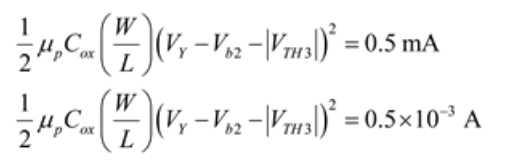
\includegraphics{3.29-13}
	\end{minipage}
\end{figure}


		\begin{figure}[H] %H为当前位置,!htb为忽略美学标准,htbp为浮动图形
	\begin{minipage}{\linewidth}
		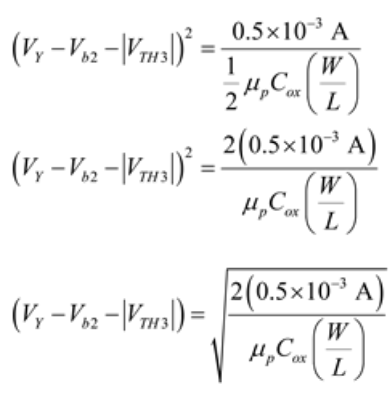
\includegraphics{3.29-14}
	\end{minipage}
\end{figure}

由$M_4$

		\begin{figure}[H] %H为当前位置,!htb为忽略美学标准,htbp为浮动图形
	\begin{minipage}{\linewidth}
		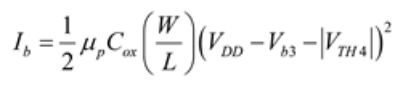
\includegraphics{3.29-15}
	\end{minipage}
\end{figure}

		\begin{figure}[H] %H为当前位置,!htb为忽略美学标准,htbp为浮动图形
	\begin{minipage}{\linewidth}
		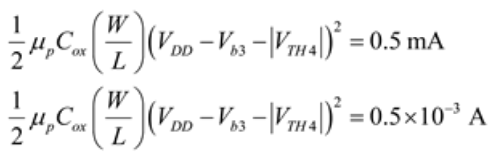
\includegraphics{3.29-16}
	\end{minipage}
\end{figure}

		\begin{figure}[H] %H为当前位置,!htb为忽略美学标准,htbp为浮动图形
	\begin{minipage}{\linewidth}
		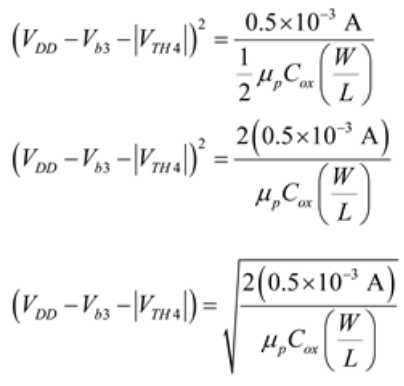
\includegraphics{3.29-17}
	\end{minipage}
\end{figure}


输出摆幅表达式

		\begin{figure}[H] %H为当前位置,!htb为忽略美学标准,htbp为浮动图形
	\begin{minipage}{\linewidth}
		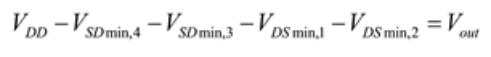
\includegraphics{3.29-18}
	\end{minipage}
\end{figure}

		\begin{figure}[H] %H为当前位置,!htb为忽略美学标准,htbp为浮动图形
	\begin{minipage}{\linewidth}
		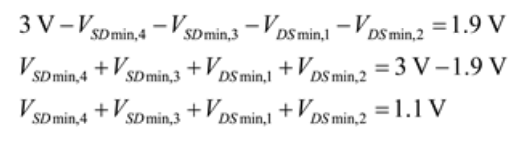
\includegraphics{3.29-19}
	\end{minipage}
\end{figure}

用临界条件$V_{GS}=|V_{DS}|$改写为

		\begin{figure}[H] %H为当前位置,!htb为忽略美学标准,htbp为浮动图形
	\begin{minipage}{\linewidth}
		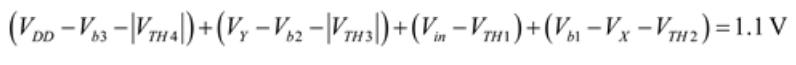
\includegraphics[width=1\linewidth]{3.29-20}
	\end{minipage}
\end{figure}

代入之前得到的结果

		\begin{figure}[H] %H为当前位置,!htb为忽略美学标准,htbp为浮动图形
	\begin{minipage}{\linewidth}
		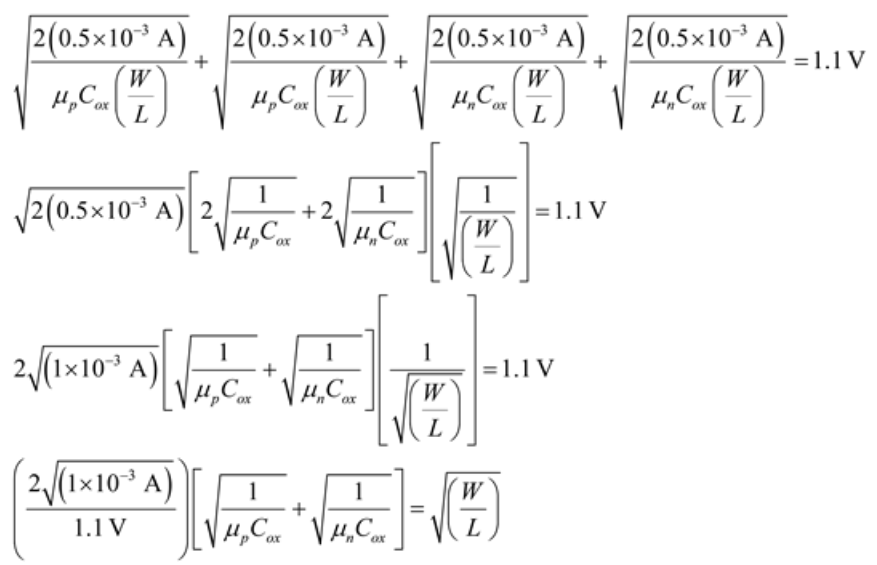
\includegraphics[width=1\linewidth]{3.29-21}
	\end{minipage}
\end{figure}

		\begin{figure}[H] %H为当前位置,!htb为忽略美学标准,htbp为浮动图形
	\begin{minipage}{\linewidth}
		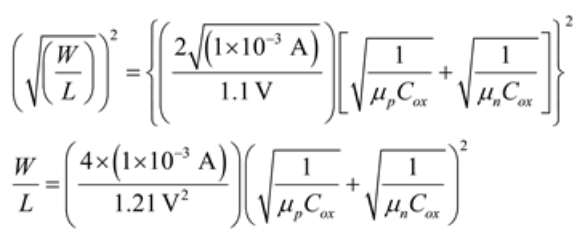
\includegraphics{3.29-22}
	\end{minipage}
\end{figure}

		\begin{figure}[H] %H为当前位置,!htb为忽略美学标准,htbp为浮动图形
	\begin{minipage}{\linewidth}
		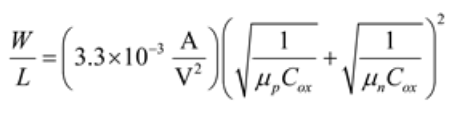
\includegraphics{3.29-23}
	\end{minipage}
\end{figure}

下面算$C_{ox}$

		\begin{figure}[H] %H为当前位置,!htb为忽略美学标准,htbp为浮动图形
	\begin{minipage}{\linewidth}
		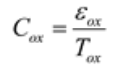
\includegraphics{3.29-24}
	\end{minipage}
\end{figure}

		\begin{figure}[H] %H为当前位置,!htb为忽略美学标准,htbp为浮动图形
	\begin{minipage}{\linewidth}
		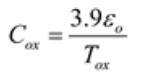
\includegraphics{3.29-25}
	\end{minipage}
\end{figure}

		\begin{figure}[H] %H为当前位置,!htb为忽略美学标准,htbp为浮动图形
	\begin{minipage}{\linewidth}
		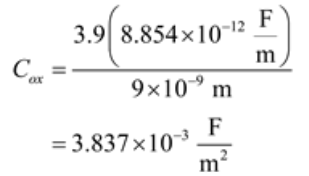
\includegraphics{3.29-26}
	\end{minipage}
\end{figure}

现在可以继续算宽长比

		\begin{figure}[H] %H为当前位置,!htb为忽略美学标准,htbp为浮动图形
	\begin{minipage}{\linewidth}
		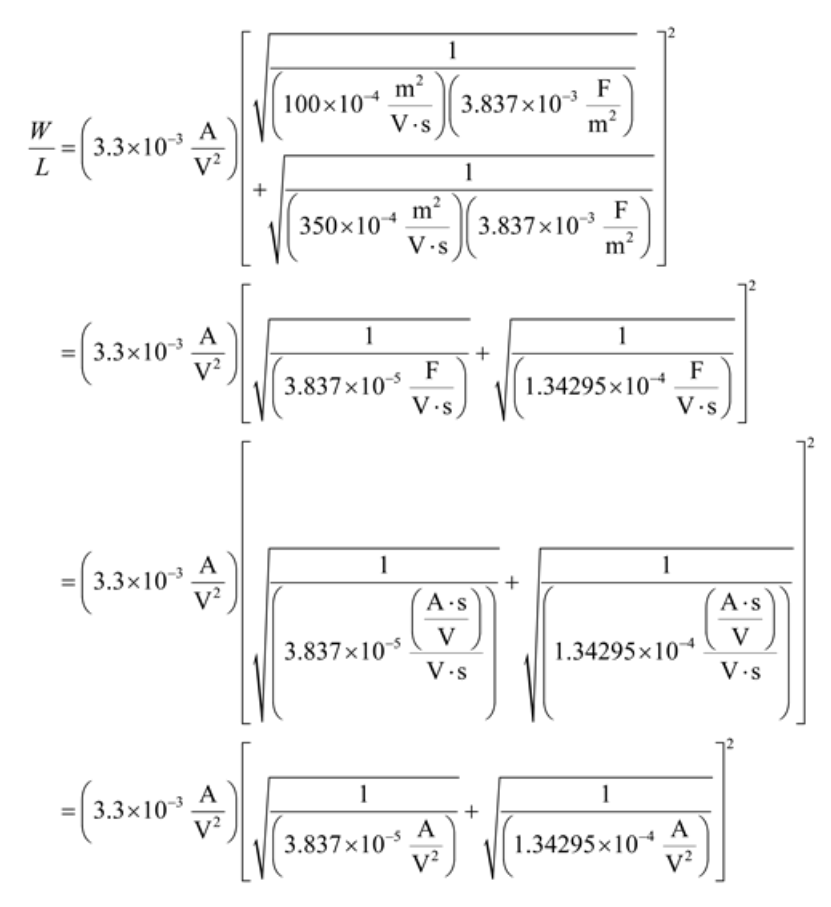
\includegraphics[width=1\linewidth]{3.29-27}
	\end{minipage}
\end{figure}

		\begin{figure}[H] %H为当前位置,!htb为忽略美学标准,htbp为浮动图形
	\begin{minipage}{\linewidth}
		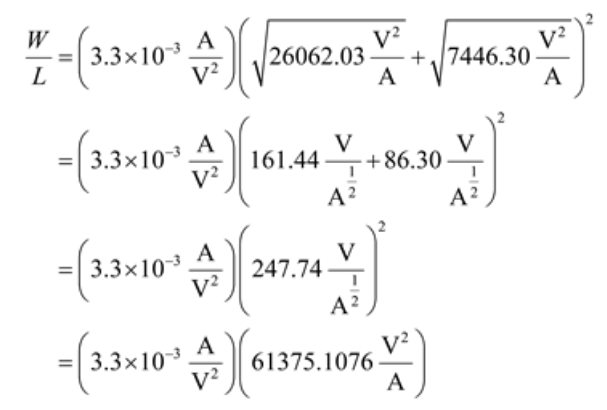
\includegraphics{3.29-28}
	\end{minipage}
\end{figure}

		\begin{figure}[H] %H为当前位置,!htb为忽略美学标准,htbp为浮动图形
	\begin{minipage}{\linewidth}
		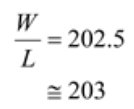
\includegraphics{3.29-29}
	\end{minipage}
\end{figure}

下面算电压

		\begin{figure}[H] %H为当前位置,!htb为忽略美学标准,htbp为浮动图形
	\begin{minipage}{\linewidth}
		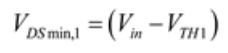
\includegraphics{3.29-30}
	\end{minipage}
\end{figure}

		\begin{figure}[H] %H为当前位置,!htb为忽略美学标准,htbp为浮动图形
	\begin{minipage}{\linewidth}
		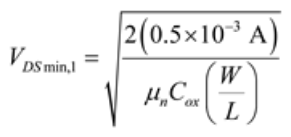
\includegraphics{3.29-31}
	\end{minipage}
\end{figure}

		\begin{figure}[H] %H为当前位置,!htb为忽略美学标准,htbp为浮动图形
	\begin{minipage}{\linewidth}
		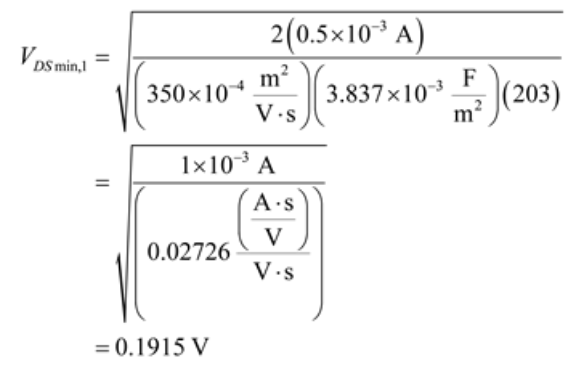
\includegraphics{3.29-32}
	\end{minipage}
\end{figure}

		\begin{figure}[H] %H为当前位置,!htb为忽略美学标准,htbp为浮动图形
	\begin{minipage}{\linewidth}
		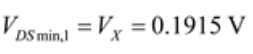
\includegraphics{3.29-33}
	\end{minipage}
\end{figure}

		\begin{figure}[H] %H为当前位置,!htb为忽略美学标准,htbp为浮动图形
	\begin{minipage}{\linewidth}
		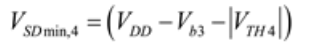
\includegraphics{3.29-34}
	\end{minipage}
\end{figure}

		\begin{figure}[H] %H为当前位置,!htb为忽略美学标准,htbp为浮动图形
	\begin{minipage}{\linewidth}
		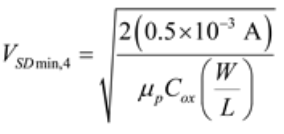
\includegraphics{3.29-35}
	\end{minipage}
\end{figure}

		\begin{figure}[H] %H为当前位置,!htb为忽略美学标准,htbp为浮动图形
	\begin{minipage}{\linewidth}
		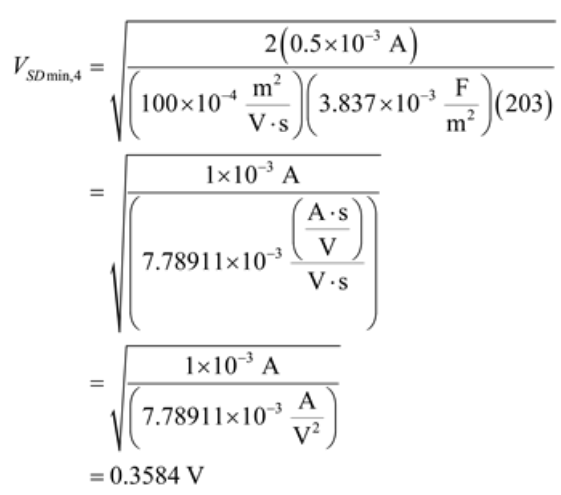
\includegraphics{3.29-36}
	\end{minipage}
\end{figure}

		\begin{figure}[H] %H为当前位置,!htb为忽略美学标准,htbp为浮动图形
	\begin{minipage}{\linewidth}
		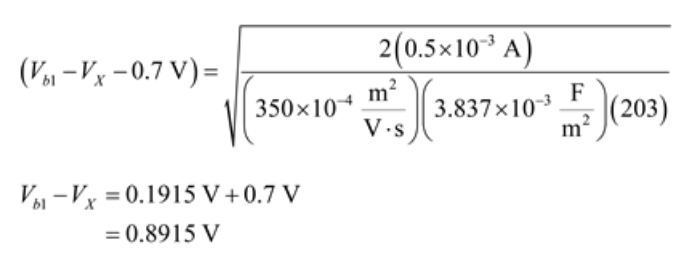
\includegraphics{3.29-37}
	\end{minipage}
\end{figure}

		\begin{figure}[H] %H为当前位置,!htb为忽略美学标准,htbp为浮动图形
	\begin{minipage}{\linewidth}
		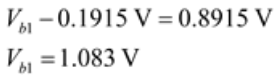
\includegraphics{3.29-38}
	\end{minipage}
\end{figure}

		\begin{figure}[H] %H为当前位置,!htb为忽略美学标准,htbp为浮动图形
	\begin{minipage}{\linewidth}
		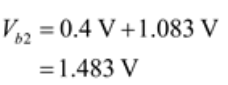
\includegraphics{3.29-39}
	\end{minipage}
\end{figure}

		\begin{figure}[H] %H为当前位置,!htb为忽略美学标准,htbp为浮动图形
	\begin{minipage}{\linewidth}
		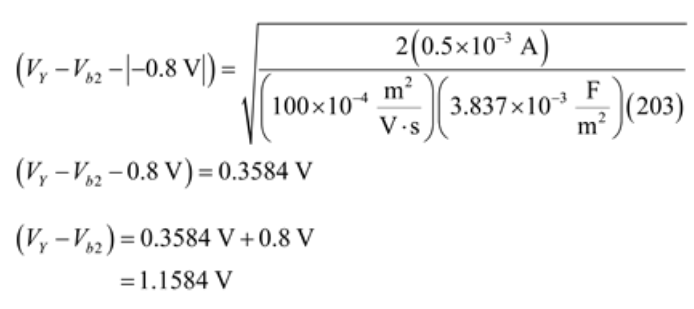
\includegraphics{3.29-40}
	\end{minipage}
\end{figure}

		\begin{figure}[H] %H为当前位置,!htb为忽略美学标准,htbp为浮动图形
	\begin{minipage}{\linewidth}
		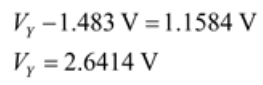
\includegraphics{3.29-41}
	\end{minipage}
\end{figure}

		\begin{figure}[H] %H为当前位置,!htb为忽略美学标准,htbp为浮动图形
	\begin{minipage}{\linewidth}
		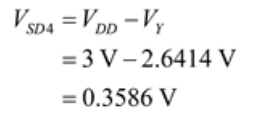
\includegraphics{3.29-42}
	\end{minipage}
\end{figure}

因此$M_1,M_2$在线性区边缘





下面算小信号电压增益

现算$M_1,M_2$的$g_m$

		\begin{figure}[H] %H为当前位置,!htb为忽略美学标准,htbp为浮动图形
	\begin{minipage}{\linewidth}
		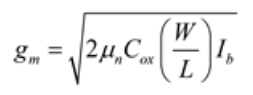
\includegraphics{3.29-43}
	\end{minipage}
\end{figure}


		\begin{figure}[H] %H为当前位置,!htb为忽略美学标准,htbp为浮动图形
	\begin{minipage}{\linewidth}
		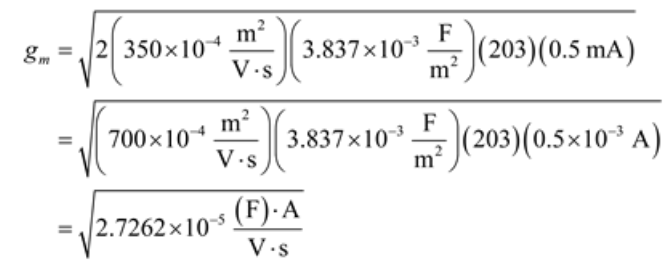
\includegraphics{3.29-44}
	\end{minipage}
\end{figure}


		\begin{figure}[H] %H为当前位置,!htb为忽略美学标准,htbp为浮动图形
	\begin{minipage}{\linewidth}
		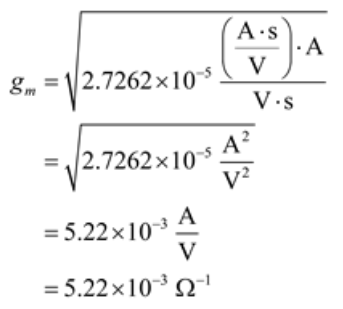
\includegraphics{3.29-45}
	\end{minipage}
\end{figure}


		\begin{figure}[H] %H为当前位置,!htb为忽略美学标准,htbp为浮动图形
	\begin{minipage}{\linewidth}
		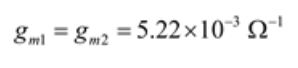
\includegraphics{3.29-46}
	\end{minipage}
\end{figure}








现算$M_3,M_4$的$g_m$

		\begin{figure}[H] %H为当前位置,!htb为忽略美学标准,htbp为浮动图形
	\begin{minipage}{\linewidth}
		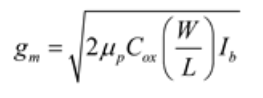
\includegraphics{3.29-47}
	\end{minipage}
\end{figure}


		\begin{figure}[H] %H为当前位置,!htb为忽略美学标准,htbp为浮动图形
	\begin{minipage}{\linewidth}
		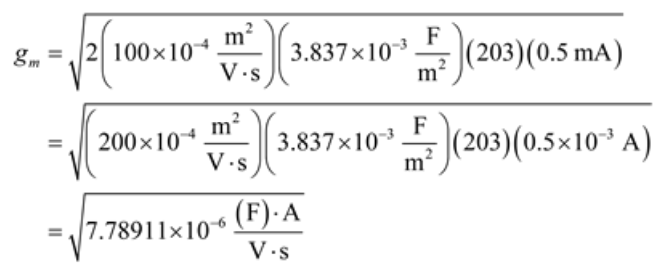
\includegraphics{3.29-48}
	\end{minipage}
\end{figure}


		\begin{figure}[H] %H为当前位置,!htb为忽略美学标准,htbp为浮动图形
	\begin{minipage}{\linewidth}
		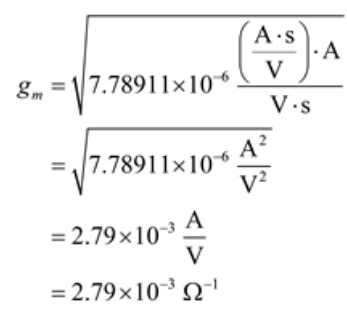
\includegraphics{3.29-49}
	\end{minipage}
\end{figure}


		\begin{figure}[H] %H为当前位置,!htb为忽略美学标准,htbp为浮动图形
	\begin{minipage}{\linewidth}
		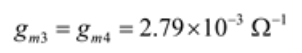
\includegraphics{3.29-50}
	\end{minipage}
\end{figure}

现算$M_1,M_2$的$r_o$

		\begin{figure}[H] %H为当前位置,!htb为忽略美学标准,htbp为浮动图形
	\begin{minipage}{\linewidth}
		\includegraphics{3.29-51}
	\end{minipage}
\end{figure}

		\begin{figure}[H] %H为当前位置,!htb为忽略美学标准,htbp为浮动图形
	\begin{minipage}{\linewidth}
		\includegraphics{3.29-52}
	\end{minipage}
\end{figure}

		\begin{figure}[H] %H为当前位置,!htb为忽略美学标准,htbp为浮动图形
	\begin{minipage}{\linewidth}
		\includegraphics{3.29-53}
	\end{minipage}
\end{figure}






现算$M_3,M_4$的$r_o$

		\begin{figure}[H] %H为当前位置,!htb为忽略美学标准,htbp为浮动图形
	\begin{minipage}{\linewidth}
		\includegraphics{3.29-54}
	\end{minipage}
\end{figure}

		\begin{figure}[H] %H为当前位置,!htb为忽略美学标准,htbp为浮动图形
	\begin{minipage}{\linewidth}
		\includegraphics{3.29-55}
	\end{minipage}
\end{figure}

		\begin{figure}[H] %H为当前位置,!htb为忽略美学标准,htbp为浮动图形
	\begin{minipage}{\linewidth}
		\includegraphics{3.29-56}
	\end{minipage}
\end{figure}

电路的等效跨导

		\begin{figure}[H] %H为当前位置,!htb为忽略美学标准,htbp为浮动图形
	\begin{minipage}{\linewidth}
		\includegraphics{3.29-57}
	\end{minipage}
\end{figure}


电路的输出电阻

$R_{out}=[(1+g_{m2}r_{o2})r_{o1}+r_{o2}]||[(1+g_{m3}r_{o3})r_{o4}+r_{o3}]$

		\begin{figure}[H] %H为当前位置,!htb为忽略美学标准,htbp为浮动图形
	\begin{minipage}{\linewidth}
		\includegraphics[width=1\linewidth]{3.29-58}
	\end{minipage}
\end{figure}

		\begin{figure}[H] %H为当前位置,!htb为忽略美学标准,htbp为浮动图形
	\begin{minipage}{\linewidth}
		\includegraphics{3.29-59}
	\end{minipage}
\end{figure}

小信号电压增益

		\begin{figure}[H] %H为当前位置,!htb为忽略美学标准,htbp为浮动图形
	\begin{minipage}{\linewidth}
		\includegraphics{3.29-60}
	\end{minipage}
\end{figure}

		\begin{figure}[H] %H为当前位置,!htb为忽略美学标准,htbp为浮动图形
	\begin{minipage}{\linewidth}
		\includegraphics{3.29-61}
	\end{minipage}
\end{figure}




